\subsection{command}
\label{subsec:command}

\begin{figure}[H]
  \centering
  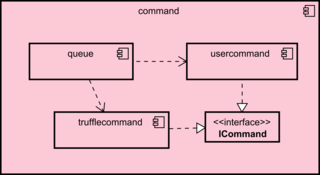
\includegraphics[width=\textwidth]{../diagramimages/command.png}
  \caption{command-Package}
\end{figure}

\medskip
Das command-Package beinhaltet alle Commands, deren Struktur, und die Datenstruktur
\textit{CommandQueue}. Ein Command ist eine Befehlssequenz, die auf
dem Model ausgeführt wird. Das heißt, alle Objekte, die das Model irgendwie verändern,
werden als Command gekapselt. Alle empfangenen Netzwerkpakete
und Benutzerbefehle werden als Command gekapselt, da diese direkt das Model beeinflussen,
indem sie im Executor ausgeführt werden.
\newline
\newline
Dieses Design hat zwei große Vorteile. Zum einen herrscht eine lose Kopplung zwischen
allen Programmteilen, welche das Model verändern wollen und dem Model selbst, was zur Modularität des
Programms beiträgt. Zum anderen kann man die Commands speichern und zu einem
späteren Zeitpunkt wieder ausführen, um zum Beispiel eine Replay-Funktion zu realisieren. Weitere Informationen dazu im
\hyperref[subsubsec:replaylogging]{replaylogging}-Package. Des Weiteren bietet dieses
Design den großen Vorteil, dass es hohes Erweiterbarkeitspotential hat. Zum Beispiel
könnte man relativ einfach eine undo- und redo-Funktion in die Commands einbauen, um
zwischen verschiedenen Modelzuständen hin und zurück zu springen, oder generell dem Benutzer zu ermöglichen, Eingaben im Programmablauf durch undo und redo zu kontrollieren. So eine
Funktionalität ist zwar vorerst nicht eingeplant, wäre durch dieses Design jedoch leicht zu implementieren.
\newline
\newline
Ein potenzielles Problem das auftreten kann, wäre, wenn ein Command zu lange braucht, um
ausgeführt zu werden und so das ganze Programm zum Stillstand kommt.
In dem jetzigen Entwurf wird dieses Problem nicht auftreten, da jeder Command
nur schnelle Befehlssequenzen ausführt, welche das System nicht
aufhängen. Wenn jedoch \gls{programname} mal so erweitert wird, dass es doch Commands gibt,
die eine lange Ausführungszeit haben, so sollten diese in seperaten Threads
ausgeführt werden um zu verhindern, dass sich das ganze Programm an einem Command
aufhängt.

Es gibt 2 Arten von Commands: TruffleCommands für die Bearbeitung empfangener
Paketdaten und UserCommands für die Verwaltung der Benutzeroberflächenbefehle.

      \subsubsection{trufflecommand}
      \label{subsubsec:trufflecommand}

      \begin{figure}[H]
        \centering
        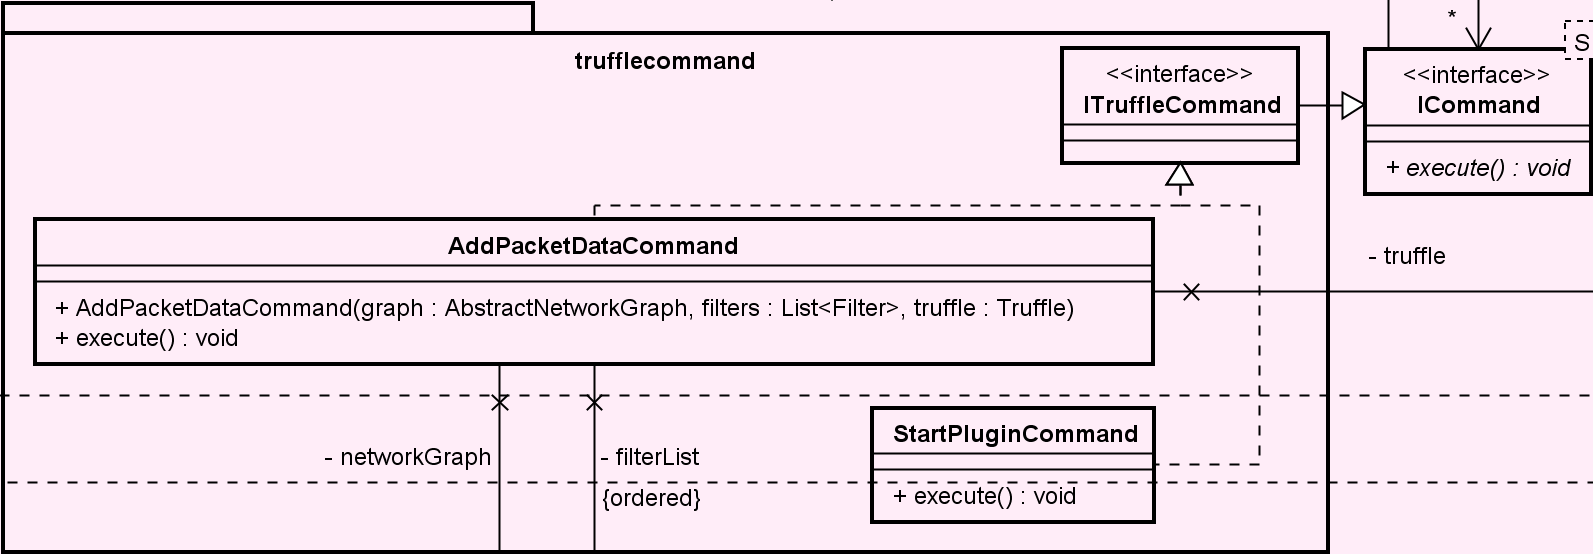
\includegraphics[width=\textwidth]{../diagramimages/trufflecommand.png}
        \caption{trufflecommand-Package}
      \end{figure}

      \medskip
      Jegliche vom \gls{praeprozessor} empfangenen \glspl{truffle} werden zuerst in Java-Objekt-\glspl{truffle} umgewandelt. (Siehe
      \hyperref[subsubsec:truffleprocessor]{truffleprocessor}-Package) Anschließend
      werden die erzeugten Java-\glspl{truffle} einem Command übergeben und per \gls{observerpattern}
      (Siehe \hyperref[subsec:util]{util}-Package) an alle Interessenten, also die \gls{listener}, verschickt.
      \newline
      \newline
      Es gibt nur einen Command-Typen für die empfangen \gls{truffle}-\glspl{paket}: Den
      AddPacketDataCommand. Es wäre nicht sinngemäß, mehrere Commands für die Funktionalität
      dieses Commands zu verwenden. Wenn man zum Beispiel mehrere Commands für das Bearbeiten von
      verschiedenen Daten hätte, so müssten in jedem Command anfragen an den Graph gestellt werden.
      Erledigt man alles in einem Command, so verringert sich die Anzahl der Aufrufe an den Graphen,
      was der Performance zugunsten kommt.
      \newline
      \newline
      Der PluginNotRunningCommand wird genau dann vom TrufflProcessor verschickt, wenn sich \gls{programname} nicht mit \gls{sppname} oder einem äquivalenten Plugin verbinden konnte. Die Funktionalität des automatisch startenden \gls{sppname} wird nicht integriert, um die beiden Programme unabhängiger zu gestalten, und dem Benutzer mehr Freiheit, beispielsweise bei der Wahl des \gls{praeprozessor}s, zu ermöglichen.

      \subsubsection{usercommand}
      \label{subsubsec:usercommand}

      \begin{figure}[H]
        \centering
        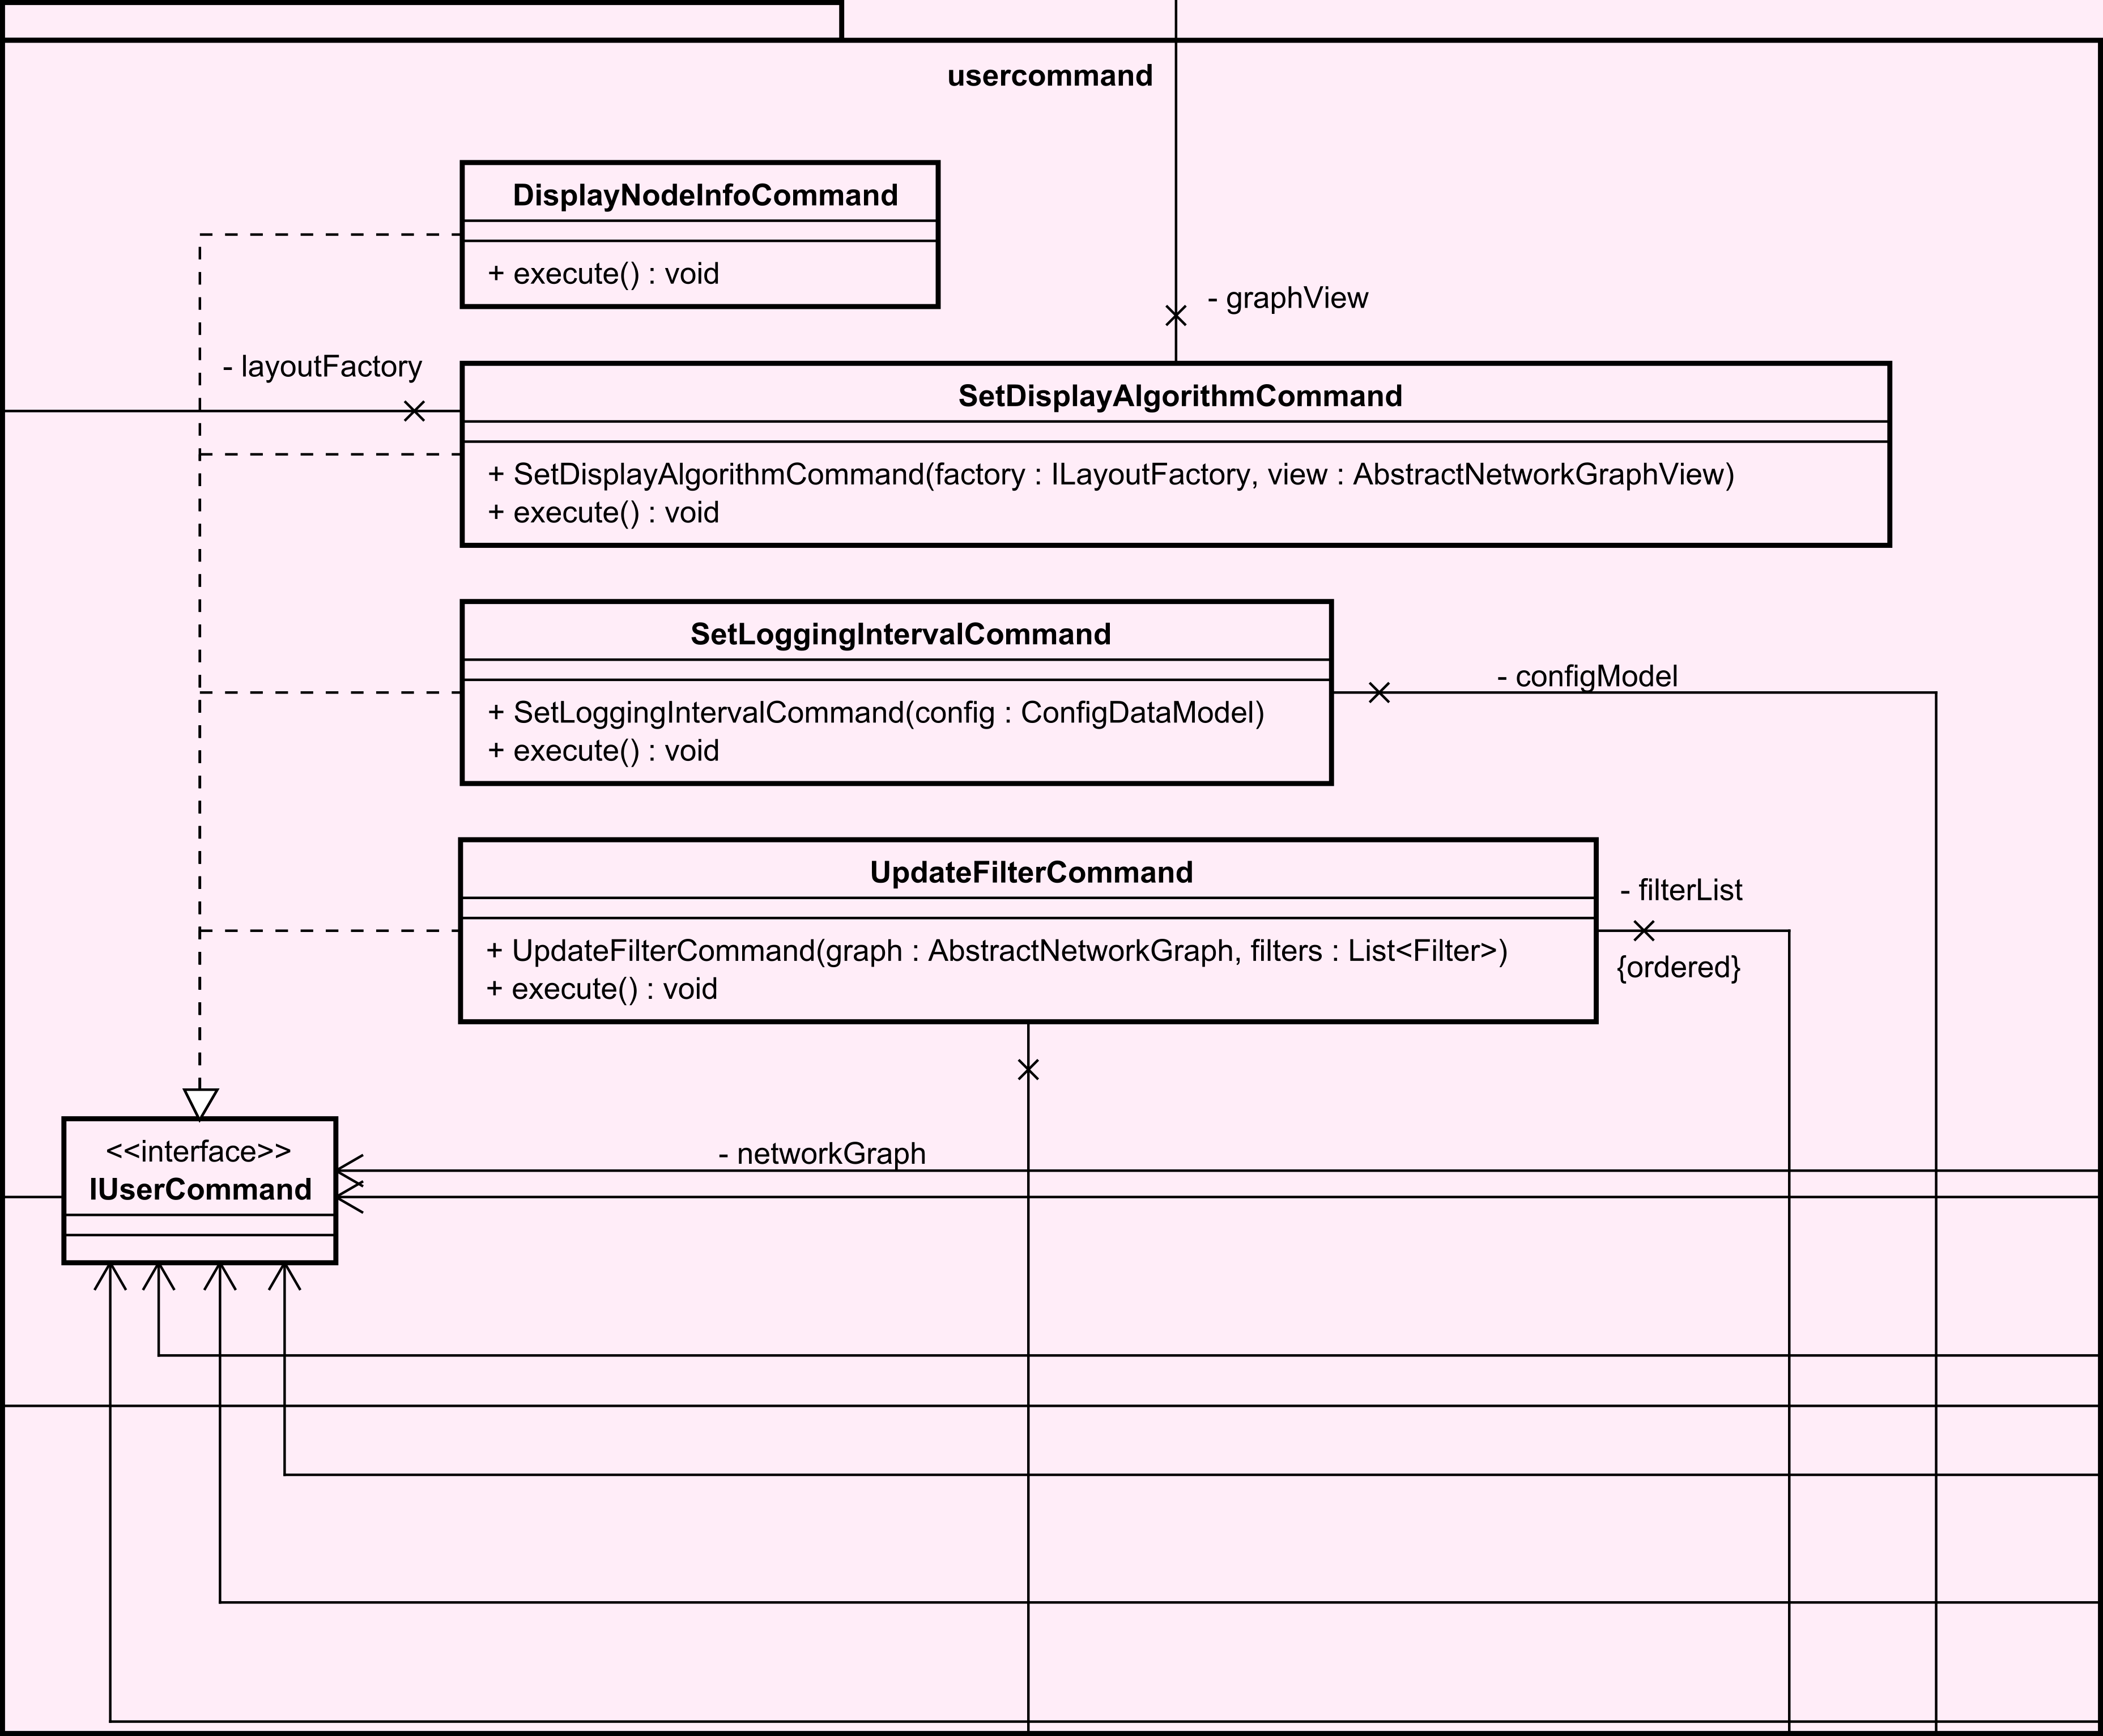
\includegraphics[width=\textwidth]{../diagramimages/usercommand.png}
        \caption{usercommand-Package}
      \end{figure}

      \medskip
      Wenn der Benutzer eine \gls{gui}-Aktion startet, die das Model beeinflusst,
      wird mittels des \gls{observerpattern}s ein entsprechender Command an alle \gls{listener} verschickt. Für jede mögliche
      \gls{gui}-Aktion gibt es einen passenden Command.
      Diese werden in den ViewControllern aus dem \hyperref[subsec:view]{view}-Package, wieder nach \gls{observerpattern},
      an den Executor verschickt.

      \subsubsection{queue}
      \label{subsubsec:queue}

      \begin{figure}[H]
        \centering
        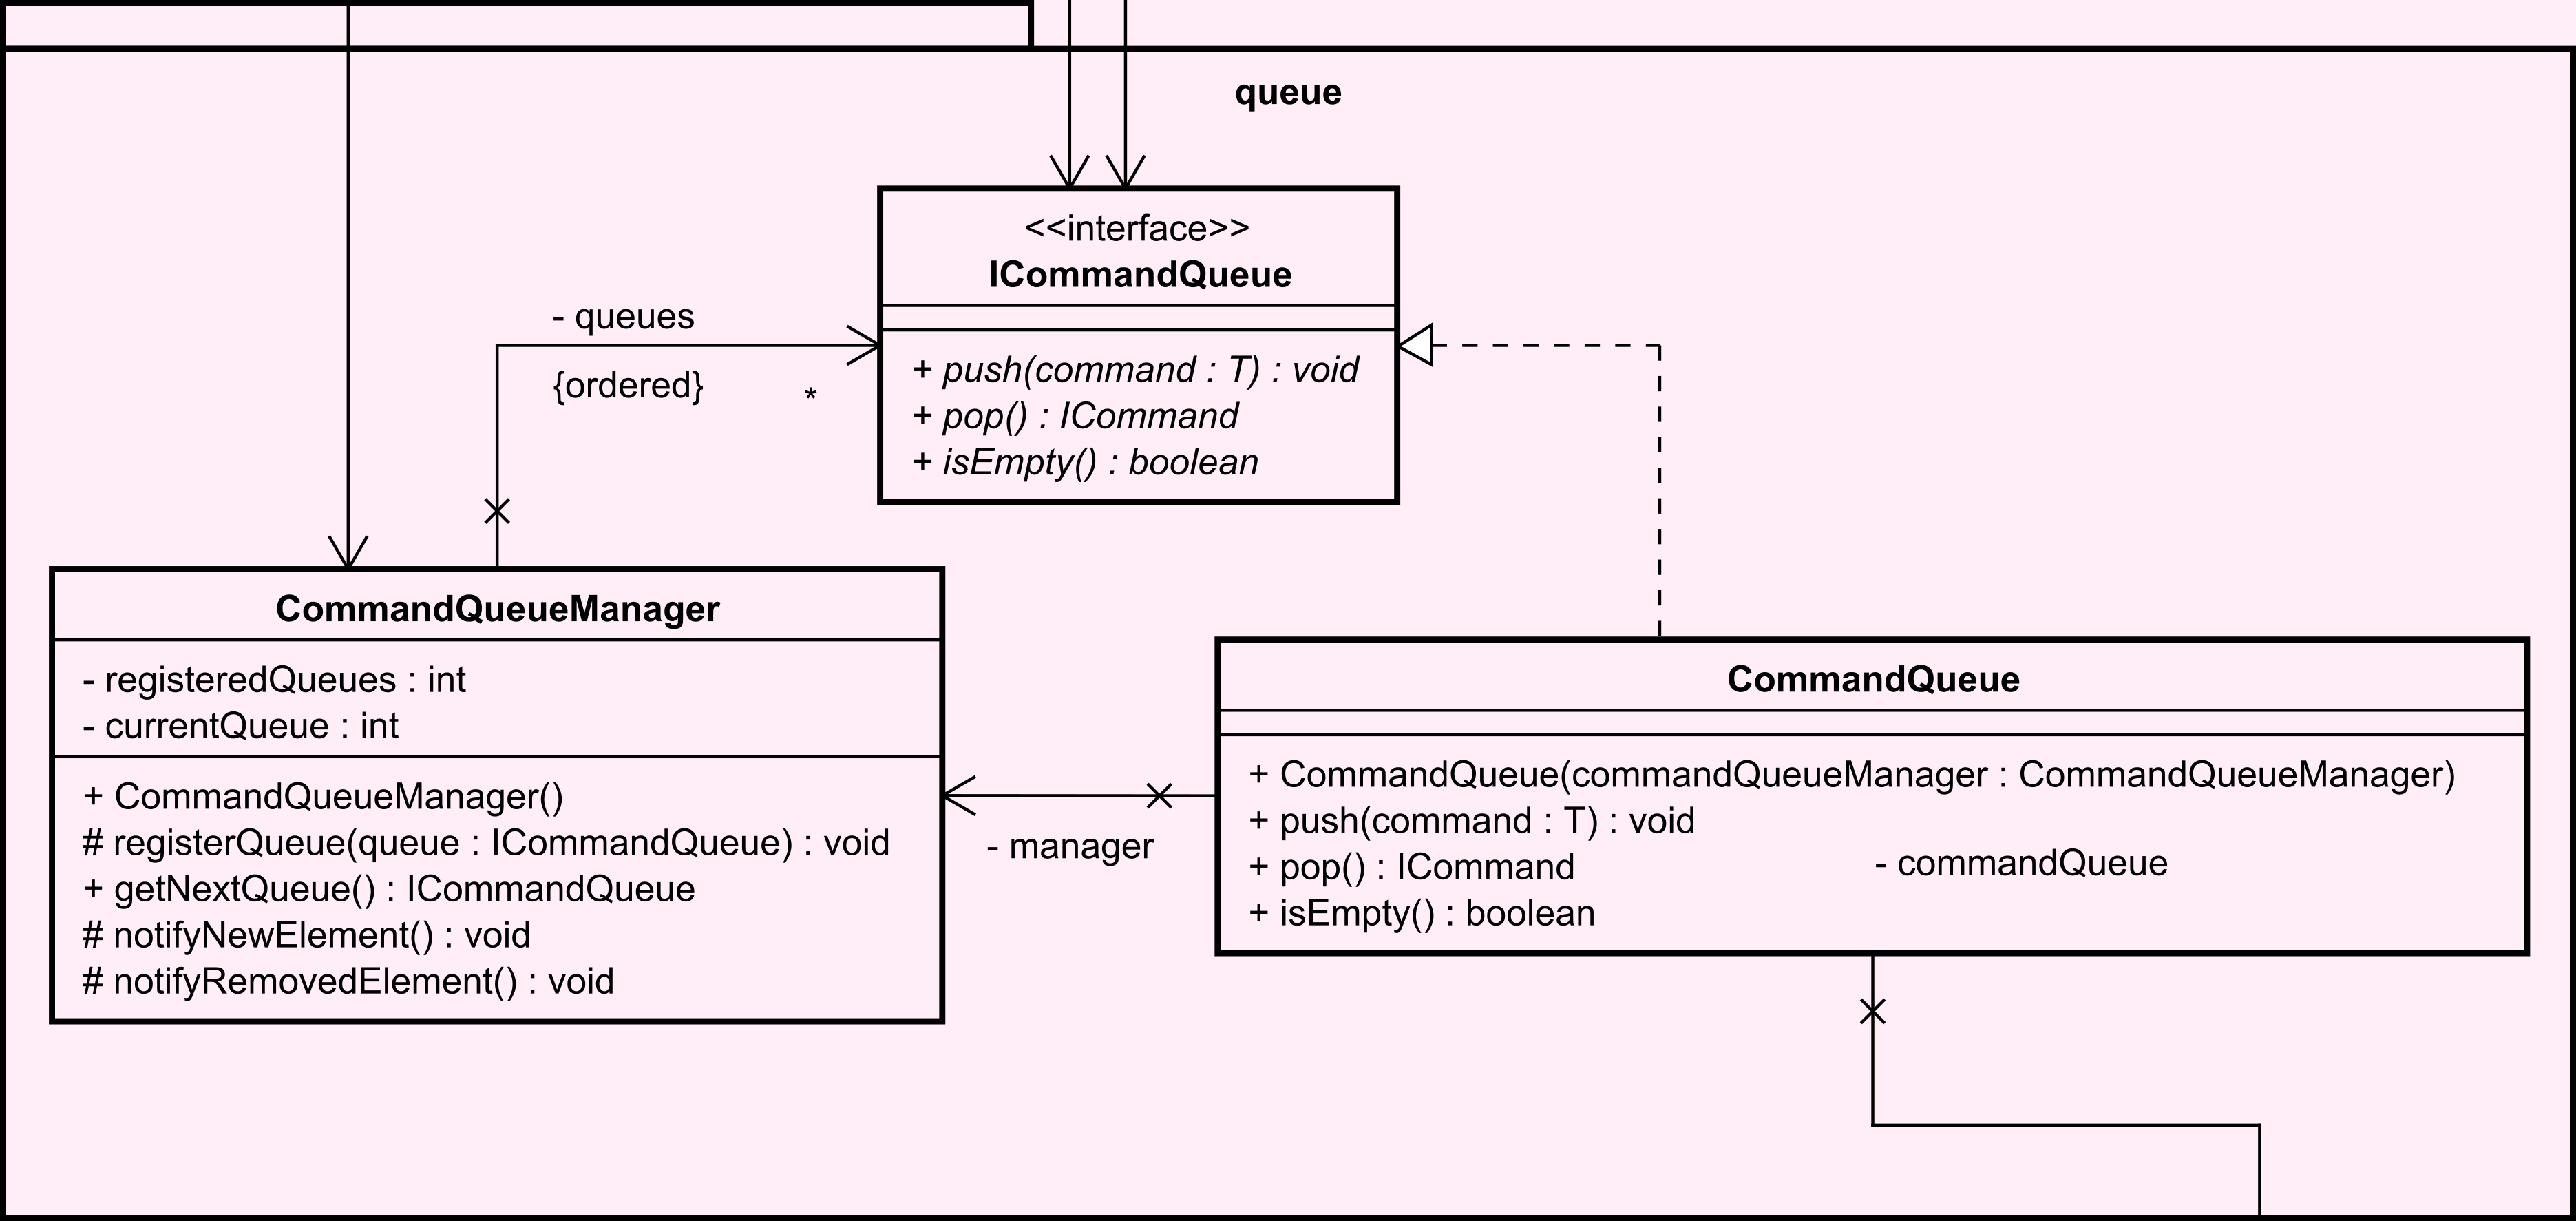
\includegraphics[width=\textwidth]{../diagramimages/queue.png}
        \caption{queue-Package}
      \end{figure}

      \medskip
      Die Commands, welche beispielsweise der Executor abarbeiten soll, werden in
      einer passenden Datenstruktur zwischengespeichert. Es sind gegebenenfalls mehrere
      tatsächliche Queues vorhanden, was nach einem Manager verlangt, um nach dem
      Round-Robin-Prinzip faire Abarbeitung zu ermöglichen. Die CommandQueue
      ist das empfangende Ende des \gls{observerpattern}s an mehreren Stellen unseres
      Programms. Bei Aktualisierung durch einen \gls{notifier} geht dieser alle
      seine \gls{listener} durch und fügt bei jedem in genau einer diese
      CommandQueue das neue Command-Objekt ein.